\documentclass[11pt,a4paper]{article}
\usepackage[margin=2.4cm]{geometry}
\usepackage{fontspec}
\usepackage{amsmath,amssymb,amsthm}
\usepackage{tikz}
\usetikzlibrary{arrows.meta,positioning,calc,matrix}
\usepackage{fancyvrb}
\usepackage{booktabs,array,tabularx}
\usepackage{xcolor}
\usepackage{stmaryrd}
\usepackage[colorlinks=true,linkcolor=blue!50!black,citecolor=blue!50!black,urlcolor=blue!50!black]{hyperref}

\setmonofont{Menlo}[Scale=0.82]
\usepackage{newunicodechar}
\newfontfamily\fbfont{Arial Unicode MS}[Scale=0.82]
\newfontfamily\fbsym{Apple Symbols}[Scale=0.9]
\newunicodechar{ᗮ}{\textsuperscript{\fbfont\symbol{"22A5}}}
\newunicodechar{⊓}{{\fbfont ⊓}}
\newunicodechar{⊔}{{\fbfont ⊔}}
\newunicodechar{⊥}{{\fbfont ⊥}}
\newunicodechar{ₖ}{\textsubscript{k}}


\definecolor{leanbg}{RGB}{246,246,250}
\definecolor{zcol}{RGB}{31,94,168}
\definecolor{xcol}{RGB}{200,70,40}
\fvset{fontsize=\footnotesize,frame=single,framesep=2mm,rulecolor=\color{black!25}}
\newcommand{\lean}[1]{\VerbatimInput{snippets/#1.lean}}
\newcommand{\lname}[1]{\texttt{\detokenize{#1}}}

\theoremstyle{plain}
\newtheorem{theorem}{Theorem}
\newtheorem{proposition}[theorem]{Proposition}
\newtheorem{lemma}[theorem]{Lemma}
\newtheorem{corollary}[theorem]{Corollary}
\theoremstyle{definition}
\newtheorem{definition}[theorem]{Definition}
\theoremstyle{remark}
\newtheorem*{remark}{Remark}

\newcommand{\C}{\mathbb{C}}
\newcommand{\ket}[1]{|#1\rangle}
\newcommand{\bra}[1]{\langle #1|}
\newcommand{\Zp}{Z_{+}}\newcommand{\Zm}{Z_{-}}\newcommand{\Xp}{X_{+}}\newcommand{\Xm}{X_{-}}
\newcommand{\Lsub}{\mathcal{L}(\C^2)}

\title{When proof by cases fails:\\ classical and quantum logic for spins, checked in Lean}
\author{Lina Alasfar\thanks{Prepared with the assistance of Claude Science, Opus 5.5 model (Anthropic). Lean proofs and source: \url{https://github.com/alasfar-lina/quantum-logic-spins-lean}.}}
\date{Lecture notes, October 2026}

\sloppy\emergencystretch=3em
\begin{document}
\maketitle

\begin{abstract}
In classical logic, ``$p$ and ($q$ or $r$)'' means the same as ``($p$ and $q$) or ($p$ and $r$)''. As a consequence, any statement can be proved by splitting into the cases $q$ and $\neg q$. We show that this rule fails for the spin of an electron, and that it fails in a precise, provable way. The failure is \emph{not} that ``$p$ or not $p$'' stops being true; it remains true. What fails is \emph{bivalence}: a state can make ``$p$ or not $p$'' true while making neither $p$ nor not-$p$ true. Intuitionistic logic, by contrast, gives up ``$p$ or not $p$'' itself. The difference traces back to the meaning of ``or'': set union classically, span in von Neumann's formalism. A closing note relates this to Aristotle's laws of thought. We then show what replaces it. Quantum propositions form an \emph{orthomodular lattice}, in which classical reasoning is still valid between compatible propositions. With two spins, the Peres--Mermin square shows the stronger result: no classical assignment of pre-existing values can reproduce quantum mechanics at all. This is the Kochen--Specker theorem. Every theorem in these notes is stated and proved in Lean~4 with Mathlib. The proof file is \texttt{QuantumLogicSpins.lean}, and Lean names are given in the margin of each statement.
\end{abstract}

\section{Classical propositions}

A classical system is, at each moment, in one state $\omega$ of a set $\Omega$ of states. A yes/no question about the system (a \emph{proposition}) is identified with the set of states for which the answer is ``yes''. ``And'', ``or'' and ``not'' then become intersection, union and complement:
\[
  P\wedge Q = P\cap Q,\qquad P\vee Q = P\cup Q,\qquad \neg P = \Omega\setminus P .
\]
The same picture covers any \emph{hidden-variable} account of quantum mechanics, in which $\omega$ is a hidden state that fixes every measurement outcome in advance.

\begin{theorem}[Distributivity and proof by cases]\label{thm:classical}
For all propositions $p,q,r$,
\[
 p\wedge(q\vee r)\;\Longleftrightarrow\;(p\wedge q)\vee(p\wedge r),
 \qquad
 p\;\Longleftrightarrow\;(p\wedge q)\vee(p\wedge\neg q).
\]
The same identities hold in every Boolean algebra, and in particular for sets of hidden states, $P=(P\cap Q)\cup(P\cap Q^{c})$. For any probability measure $\mu$ (law of total probability),
\[
\mu(P\cap Q)+\mu(P\cap Q^{c})=\mu(P).
\]
\end{theorem}
\noindent Lean: \lname{classical_distrib}, \lname{classical_case_split}, \lname{boolean_case_split}, \lname{hidden_variable_case_split}, \lname{classical_total_probability}.
\lean{classical_distrib}
\lean{classical_case_split}
\lean{classical_total_probability}

\begin{remark}
Lean's \texttt{\#print axioms} shows a difference between the two classical laws. Distributivity needs no axioms. Proof by cases uses \texttt{Classical.choice}, which is how Lean provides the law of excluded middle. Lean's core logic is intuitionistic, and excluded middle is added as an axiom. So proof by cases rests on two ingredients: excluded middle, and the step from ``$q\vee\neg q$ is true'' to ``$q$ is true, or $\neg q$ is true''. Intuitionistic logic drops the first. Quantum logic keeps the first and drops the second (Section~\ref{sec:biv}).
\end{remark}

\section{One spin}

\subsection{Quantum propositions}
The spin of an electron is described by unit vectors in $\C^2$, up to a phase. Write
\[
 \ket{z{+}}=\begin{pmatrix}1\\0\end{pmatrix},\quad
 \ket{z{-}}=\begin{pmatrix}0\\1\end{pmatrix},\quad
 \ket{x{\pm}}=\tfrac{1}{\sqrt2}\begin{pmatrix}1\\\pm1\end{pmatrix},
\]
the states in which $S_z$ or $S_x$ certainly takes the value $\pm\hbar/2$.

\begin{definition}[Birkhoff--von Neumann]
A proposition about the spin is a (closed) linear subspace $P\subseteq\C^2$: the set of states for which the answer is certainly ``yes''. The connectives are
\[
 P\wedge Q=P\cap Q,\qquad P\vee Q=P+Q=\operatorname{span}(P\cup Q),\qquad \neg P=P^{\perp}.
\]
We write $\Lsub$ for the set of all such propositions, $0=\{0\}$ for ``absurd'' and $\C^2$ for ``always true''. The four propositions of interest are the lines
$\Zp=\C\ket{z{+}}$, $\Zm=\C\ket{z{-}}$, $\Xp=\C\ket{x{+}}$, $\Xm=\C\ket{x{-}}$.
\end{definition}

The only change from the classical case is ``or''. The union of two lines is not a subspace. A superposition of a state in $P$ and a state in $Q$ is a legitimate state, so $P\vee Q$ must contain the whole span. In Lean, $\Lsub$ is Mathlib's lattice \texttt{Submodule ℂ (EuclideanSpace ℂ (Fin 2))}, with $\perp$ the orthogonal complement \texttt{Kᗮ}. Normalisation does not change a line, so the file uses $(1,\pm1)$ for $\ket{x{\pm}}$.
\lean{defs_spin}

\begin{lemma}[Two directions]\label{lem:lines}
If $u,v\in\C^2$ are not parallel ($u_0v_1-u_1v_0\neq0$), then $\C u\wedge\C v=0$ and $\C u\vee\C v=\C^2$. If in addition $u\perp v$, then $\neg(\C u)=\C v$.
\end{lemma}
\noindent Lean: \lname{lines_inf}, \lname{lines_sup}, \lname{orth_line}. Applied to the spin states, this gives $\Zp\wedge\Xp=\Zp\wedge\Xm=\Zm\wedge\Xp=\Zm\wedge\Xm=0$, $\Zp\vee\Zm=\Xp\vee\Xm=\C^2$, $\neg\Zp=\Zm$ and $\neg\Xp=\Xm$. In words: no state has a definite $S_z$ and a definite $S_x$ at the same time, but each of $S_z$ and $S_x$ certainly has \emph{some} value.

\begin{figure}[t]
\centering
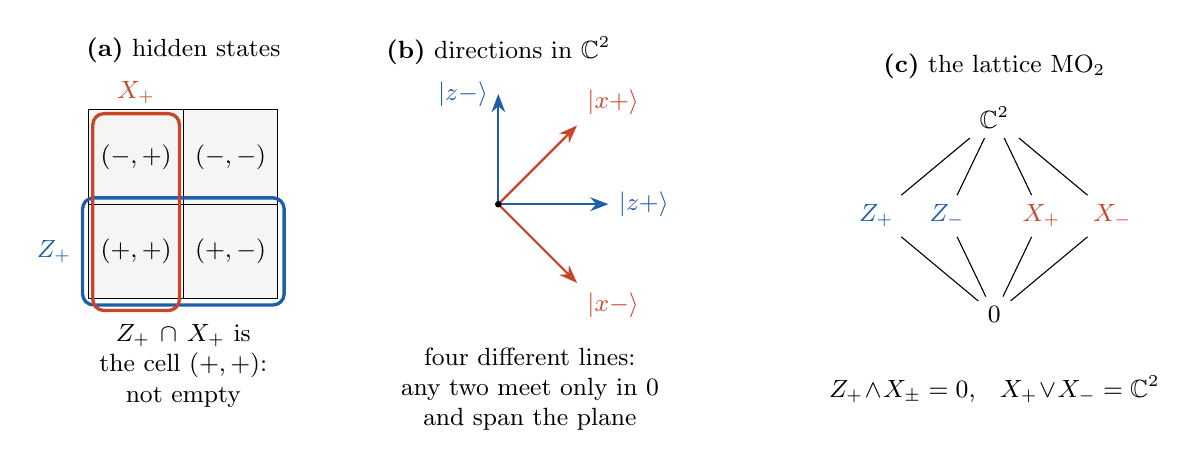
\begin{tikzpicture}[scale=1.0, every node/.style={font=\small}]
% (a) classical hidden states
\begin{scope}
 \node at (1.2,3.55) {\textbf{(a)} hidden states};
 \foreach \i/\sx in {0/+,1/-} \foreach \j/\sz in {0/+,1/-} {
   \draw[fill=black!4] (1.2*\i,1.2*\j+0.4) rectangle ++(1.2,1.2);
   \node at (1.2*\i+0.6,1.2*\j+1.0) {$(\sz,\sx)$};
 }
 \draw[zcol,very thick,rounded corners] (-0.08,0.32) rectangle (2.48,1.68);
 \node[zcol,left] at (-0.1,1.0) {$Z_+$};
 \draw[xcol,very thick,rounded corners] (0.05,0.25) rectangle (1.15,2.75);
 \node[xcol,above] at (0.6,2.75) {$X_+$};
 \node[align=center,text width=3.6cm] at (1.2,-0.45) {$Z_+\cap X_+$ is the cell $(+,+)$:\\ not empty};
\end{scope}
% (b) the plane
\begin{scope}[xshift=5.2cm,yshift=1.6cm]
 \node at (0,1.95) {\textbf{(b)} directions in $\C^2$};
 \draw[-{Stealth},zcol,thick] (0,0) -- (1.4,0) node[right]{$\ket{z{+}}$};
 \draw[-{Stealth},zcol,thick] (0,0) -- (0,1.4) node[left]{$\ket{z{-}}$};
 \draw[-{Stealth},xcol,thick] (0,0) -- (1.0,1.0) node[above right]{$\ket{x{+}}$};
 \draw[-{Stealth},xcol,thick] (0,0) -- (1.0,-1.0) node[below right]{$\ket{x{-}}$};
 \fill (0,0) circle (1.2pt);
 \node[align=center,text width=3.8cm] at (0.4,-2.35) {four different lines:\\ any two meet only in $0$\\ and span the plane};
\end{scope}
% (c) Hasse diagram MO2
\begin{scope}[xshift=10.6cm,yshift=0.2cm]
 \node at (0.9,3.15) {\textbf{(c)} the lattice MO$_2$};
 \node (top) at (0.9,2.5) {$\C^2$};
 \node (bot) at (0.9,0) {$0$};
 \node[zcol] (zp) at (-0.6,1.25) {$Z_+$};
 \node[zcol] (zm) at (0.3,1.25) {$Z_-$};
 \node[xcol] (xp) at (1.5,1.25) {$X_+$};
 \node[xcol] (xm) at (2.4,1.25) {$X_-$};
 \foreach \n in {zp,zm,xp,xm} { \draw (bot) -- (\n); \draw (\n) -- (top); }
 \node[align=center,text width=4.2cm] at (0.9,-0.95) {$Z_+\wedge X_\pm=0$, \; $X_+\vee X_-=\C^2$};
\end{scope}
\end{tikzpicture}
\caption{(a) In a hidden-variable picture every state fixes both $S_z$ and $S_x$, so ``$S_z=+$ and $S_x=+$'' is a non-empty set. (b) For a spin, the four propositions are four lines in $\C^2$ (real slice shown). (c) The six propositions $0,\Zp,\Zm,\Xp,\Xm,\C^2$ form the lattice MO$_2$. It is the union of two Boolean blocks (blue: $S_z$; red: $S_x$) glued at $0$ and $\C^2$.}
\label{fig:mo2}
\end{figure}

\subsection{Excluded middle versus bivalence}\label{sec:biv}
Two principles that coincide in classical logic come apart here.
\begin{description}
\item[Excluded middle] For every proposition $P$, the proposition $P\vee\neg P$ is always true.
\item[Bivalence] For every proposition $P$ and every state $\psi$, either $\psi$ makes $P$ true or $\psi$ makes $\neg P$ true. Equivalently, a true ``or'' always has a true part.
\end{description}
For sets of states (Fig.~\ref{fig:biv}a) the two principles say the same thing, because every point lies in $P$ or in its complement. For spin propositions they differ.

\begin{theorem}[Excluded middle holds, bivalence fails]\label{thm:biv}
For every $P\in\Lsub$, $P\vee\neg P=\C^2$. But the state $\ket{x{+}}$ satisfies ``$S_z=+\tfrac12$ or not $S_z=+\tfrac12$'', while $\ket{x{+}}\notin\Zp$ and $\ket{x{+}}\notin(\neg\Zp)=\Zm$.
\end{theorem}
\begin{proof}
The first statement is Mathlib's $K\vee K^\perp=\C^2$ (Theorem~\ref{thm:oml} below). For the second: if $a\ket{z{+}}=(1,1)/\sqrt2$, the second component would give $0=1/\sqrt2$. Similarly, the first component rules out $\ket{x{+}}\in\Zm$.
\end{proof}
\noindent Lean: \lname{excluded_middle_but_not_bivalence}, \lname{quantum_ortholattice}.
\lean{excluded_middle_but_not_bivalence}

\begin{figure}[t]
\centering
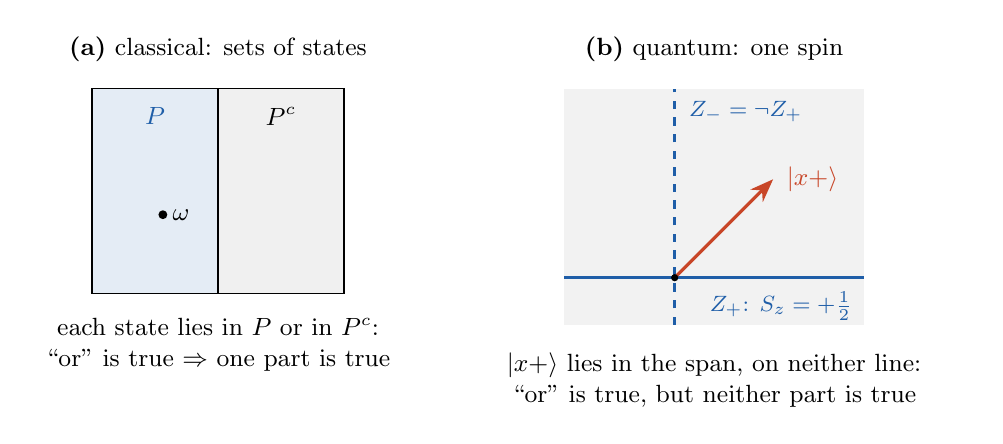
\begin{tikzpicture}[every node/.style={font=\small}]
\begin{scope}
 \node at (1.6,3.1) {\textbf{(a)} classical: sets of states};
 \fill[zcol!12] (0,0) rectangle (1.6,2.6);
 \fill[black!6] (1.6,0) rectangle (3.2,2.6);
 \draw (0,0) rectangle (3.2,2.6); \draw (1.6,0) -- (1.6,2.6);
 \node[zcol] at (0.8,2.25) {$P$}; \node at (2.4,2.25) {$P^{c}$};
 \fill (0.9,1.0) circle (1.6pt) node[right] {$\omega$};
 \node[align=center,text width=4.6cm] at (1.6,-0.65) {each state lies in $P$ or in $P^{c}$:\\ ``or'' is true $\Rightarrow$ one part is true};
\end{scope}
\begin{scope}[xshift=7.4cm,yshift=0.2cm]
 \node at (0.5,2.9) {\textbf{(b)} quantum: one spin};
 \fill[black!5] (-1.4,-0.6) rectangle (2.4,2.4);
 \draw[zcol,very thick] (-1.4,0) -- (2.4,0);
 \node[zcol,anchor=north east,font=\footnotesize] at (2.38,-0.06) {$\Zp$: $S_z=+\tfrac12$};
 \draw[zcol,very thick,dashed] (0,-0.6) -- (0,2.4);
 \node[zcol,anchor=north west,font=\footnotesize] at (0.06,2.36) {$\Zm=\neg\Zp$};
 \draw[-{Stealth},xcol,very thick] (0,0) -- (1.25,1.25);
 \node[xcol,anchor=west] at (1.3,1.25) {$\ket{x{+}}$};
 \fill (0,0) circle (1.3pt);
 \node[align=center,text width=6.4cm] at (0.5,-1.3) {$\ket{x{+}}$ lies in the span, on neither line:\\ ``or'' is true, but neither part is true};
\end{scope}
\end{tikzpicture}
\caption{Excluded middle versus bivalence. (a) Classically, every state lies in $P$ or in $P^c$. (b) For a spin, ``$S_z=+\tfrac12$ or $S_z=-\tfrac12$'' is the whole space (shaded), so every state satisfies it. Yet $\ket{x{+}}$ is on neither line, so it satisfies neither part (real slice of $\C^2$).}
\label{fig:biv}
\end{figure}

This is precisely where proof by cases breaks. From ``$q\vee\neg q$'' a classical proof goes on to ``case 1: $q$; case 2: $\neg q$''. For a spin in the state $\ket{x{+}}$, with $q$ = ``$S_z=+\tfrac12$'', neither case applies. The distributive law of the next subsection is the algebraic form of this step.

\subsection{Which ``or'', which ``not''?}\label{sec:ornot}
Comparing the two logics means comparing their connectives, and they differ in both ``or'' and ``not''.

\paragraph{``Or''.} Classically, ``$P$ or $Q$'' is the set union $P\cup Q$: the states in which at least one of the two answers is ``yes''. In von Neumann's formalism it is the span $P\vee Q$. The union of two lines is not a subspace, and the span has to contain every superposition. For $Q=P^\perp$ the two readings give opposite results, and superposition is the reason in both cases:
\[
 \Zp\cup\Zp^{\perp}\neq\C^2,
 \qquad\qquad
 P\vee P^{\perp}=\C^2\ \text{ for every } P .
\]
The left identity holds because the superposition $\ket{x{+}}=(\ket{z{+}}+\ket{z{-}})/\sqrt2$ lies on neither line. The right identity holds because the span of a line and its orthogonal line contains all such superpositions. The two logics therefore diverge even where they seem to agree. Classically, $P\cup P^{c}=\Omega$ holds \emph{because} every state lies in $P$ or in its complement. In von Neumann's logic, $P\vee P^{\perp}=\C^2$ also holds, but the classical reason is false, since $\ket{x{+}}$ lies in neither. Classically, a state makes ``$P$ or $Q$'' true only by being in $P$ or in $Q$. A quantum state can make $P\vee Q$ true while being in neither.
\begin{theorem}[Union versus span]\label{thm:unionspan}
$\Zp\cup\Zp^{\perp}\neq\C^2$ as sets, while $P\vee P^\perp=\C^2$ for every subspace $P$.
\end{theorem}
\noindent Lean: \lname{union_with_orthocomplement_not_everything}, \lname{span_with_orthocomplement_everything}.
\lean{union_with_orthocomplement_not_everything}

\paragraph{``Not''.} In a Boolean algebra, ``not'' is fixed by ``and'' and ``or''. There is exactly one $Q$ with $P\wedge Q=$ absurd and $P\vee Q=$ always true. In MO$_2$ this fails. The proposition ``$S_z=+\tfrac12$'' has three such partners: $\Zm$, $\Xp$ and $\Xm$. The lattice alone does not say which of them is ``not $S_z=+\tfrac12$''. Von Neumann's formalism supplies the missing structure, orthogonality, and chooses $\Zp^\perp=\Zm$.
\begin{proposition}[Complements are not unique]\label{prop:compl}
In MO$_2$, the elements $c$ with $\Zp\wedge c=0$ and $\Zp\vee c=\C^2$ are exactly $\Zm$, $\Xp$, $\Xm$.
\end{proposition}
\noindent Lean: \lname{MO2_complements_of_zu}, checked over all six elements by \texttt{decide}.

\paragraph{Which ``excluded middle''?} Three different statements go by this name. They should be kept apart.
\begin{enumerate}
\item \emph{The formula $p\vee\neg p$ inside the logic.} With von Neumann's span and orthocomplement it always holds (Theorem~\ref{thm:unionspan}, right).
\item \emph{``Either $p$ is true or $\neg p$ is true'' in a given state.} This is bivalence, and with set union as ``or'' it is the left identity of Theorem~\ref{thm:unionspan}. It fails for a spin. Esfahanian and Arntzen~\cite{EA} take this reading as their definition of excluded middle.
\item \emph{Excluded middle in the mathematics used to describe quantum theory.} Ref.~\cite{EA} argues that it can be dropped, building on constructive mathematics and topos theory. In the topos approach of D\"oring and Isham~\cite{DI}, quantum propositions are represented so that their logic is intuitionistic (see also~\cite{Landsman}). There the formula $p\vee\neg p$ itself fails, and in exchange the distributive law returns. This moves quantum theory from the third column of the table in Section~\ref{sec:twoways} to the second.
\end{enumerate}
The Lean file stays at level~1 for the logic of spins, and its own reasoning about spins is classical. Mathlib adds \texttt{Classical.choice} on top of Lean's intuitionistic core.

\subsection{Distributivity fails}

\begin{theorem}[Birkhoff--von Neumann]\label{thm:fail}
\[
 \Zp\wedge(\Xp\vee\neg\Xp)=\Zp,\qquad\text{but}\qquad(\Zp\wedge\Xp)\vee(\Zp\wedge\neg\Xp)=0\neq\Zp .
\]
Hence neither the distributive law nor proof by cases holds in $\Lsub$.
\end{theorem}
\begin{proof}
By Lemma~\ref{lem:lines}, $\neg\Xp=\Xm$ and $\Xp\vee\Xm=\C^2$, so the left side is $\Zp\wedge\C^2=\Zp$. Both terms on the right are $0$. The line $\Zp$ is not $0$, because $\ket{z{+}}\ne0$.
\end{proof}
\noindent Lean: \lname{spin_distributivity_fails}, \lname{subspaces_not_distributive}, \lname{quantum_case_split_fails}.
\lean{spin_distributivity_fails}
\lean{subspaces_not_distributive}

\paragraph{Physical reading.} Prepare an electron in $\ket{z{+}}$, for example with a Stern--Gerlach magnet oriented along $z$. Then ``$S_z=+\hbar/2$'' is certain. ``$S_x=+\hbar/2$ or $S_x=-\hbar/2$'' is also certain, because an $S_x$ measurement always gives one of the two values. Classically we would conclude that one of the two conjunctions ``$S_z=+$ and $S_x=+$'' or ``$S_z=+$ and $S_x=-$'' is true. But no state makes either of them true.

\begin{corollary}[No classical model]\label{cor:nohv}
\begin{enumerate}
\item There is no assignment $v:\Lsub\to\{\text{true},\text{false}\}$ with $v(\C^2)=\text{true}$, $v(0)=\text{false}$, $v(P\wedge Q)=v(P)\wedge v(Q)$ and $v(P\vee Q)=v(P)\vee v(Q)$.
\item For no set $\Omega$ is there an injective map $f:\Lsub\to 2^{\Omega}$ with $f(P\wedge Q)=f(P)\cap f(Q)$ and $f(P\vee Q)=f(P)\cup f(Q)$.
\end{enumerate}
\end{corollary}
\begin{proof}
(1) $v(\Zp)\vee v(\Zm)=v(\C^2)$ is true, and so is $v(\Xp)\vee v(\Xm)$. So some $Z_\pm$ and some $X_\pm$ are both true, but their meet is $0$, which is false. (2) Such an $f$ would carry the distributive law of sets back to $\Lsub$, contradicting Theorem~\ref{thm:fail}.
\end{proof}
\noindent Lean: \lname{no_truth_valuation}, \lname{no_hidden_variable_embedding}.
\lean{no_hidden_variable_embedding}

\section{What quantum logic keeps}

The failure is not a breakdown of logic. It replaces distributivity by a weaker law that \emph{does} hold.

\begin{theorem}[Orthomodular lattice]\label{thm:oml}
For all $K,L\in\Lsub$:
$K\wedge\neg K=0$, $K\vee\neg K=\C^2$, $\neg\neg K=K$, $K\le L\Rightarrow\neg L\le\neg K$. Also, the orthomodular law holds:
\[
 K\le L\quad\Longrightarrow\quad L=K\vee(\neg K\wedge L).
\]
\end{theorem}
\noindent Lean: \lname{quantum_ortholattice}, \lname{quantum_orthomodular}. Both follow from Mathlib's orthogonal projection, so they hold for every subspace, not only the six in Fig.~\ref{fig:mo2}. Excluded middle ($K\vee\neg K=\C^2$) and non-contradiction survive. What is lost is distributivity between \emph{incompatible} propositions.

\begin{proposition}[Classical reasoning among compatible propositions]\label{prop:compat}
If $p\le q$ or $p\le\neg q$, then $p=(p\wedge q)\vee(p\wedge\neg q)$. Within one Boolean block of MO$_2$, for example $\{0,\Zp,\Zm,\C^2\}$, the distributive law holds for all triples.
\end{proposition}
\noindent Lean: \lname{case_split_for_compatible}, \lname{MO2_z_block_distributive}.

In quantum logic, the identity $p=(p\wedge q)\vee(p\wedge\neg q)$ is taken as the \emph{definition} of ``$p$ is compatible with $q$''. Physically, compatible means jointly measurable. A Boolean algebra is the special case of an orthomodular lattice in which every pair of propositions is compatible.

\begin{proposition}[MO$_2$ is the logic of the six spin propositions]
Let MO$_2$ be the six-element lattice of Fig.~\ref{fig:mo2}(c). The map $\llbracket\cdot\rrbracket$ that sends each element to the corresponding subspace satisfies $\llbracket a\wedge b\rrbracket=\llbracket a\rrbracket\cap\llbracket b\rrbracket$, $\llbracket a\vee b\rrbracket=\llbracket a\rrbracket+\llbracket b\rrbracket$ and $\llbracket\neg a\rrbracket=\llbracket a\rrbracket^\perp$. In MO$_2$, the orthocomplement laws and the orthomodular law hold for all elements. Distributivity fails.
\end{proposition}
\noindent Lean: \lname{sem_meet}, \lname{sem_join}, \lname{sem_compl}, \lname{MO2_ortho}, \lname{MO2_orthomodular}, \lname{MO2_not_distributive}. The MO$_2$ facts are proved by \texttt{decide}, i.e.\ by checking every case, which is a useful contrast with the conceptual proofs on subspaces.

\subsection{Probabilities}
In the state $\ket{z{+}}$, the Born rule gives each proposition $P$ the probability $\mu(P)=\lVert \Pi_P\ket{z{+}}\rVert^2$, where $\Pi_P$ is the orthogonal projection onto $P$:
\begin{center}
\begin{tabular}{lcccccc}\toprule
$P$ & $0$ & $\Zp$ & $\Zm$ & $\Xp$ & $\Xm$ & $\C^2$\\\midrule
$\mu(P)$ & $0$ & $1$ & $0$ & $\tfrac12$ & $\tfrac12$ & $1$\\\bottomrule
\end{tabular}
\end{center}
with $|\langle x{+}|z{+}\rangle|^2=\tfrac12$ (Lean: \lname{born_overlap}).

\begin{proposition}\label{prop:born}
$\mu$ is a consistent probability assignment on MO$_2$: $\mu(\C^2)=1$, and $\mu(a\vee b)=\mu(a)+\mu(b)$ whenever $a\le\neg b$ (mutually exclusive propositions). Nevertheless,
\[
 \mu(\Zp)=1\;\neq\;0=\mu(\Zp\wedge\Xp)+\mu(\Zp\wedge\Xm),
\]
so the law of total probability of Theorem~\ref{thm:classical} fails.
\end{proposition}
\noindent Lean: \lname{born_is_a_state}, \lname{total_probability_fails}.

\subsection{Two ways to leave classical logic}\label{sec:twoways}
Intuitionistic and quantum logic both weaken classical logic, but in opposite places. In Lean, the intuitionistic examples use the three-valued Heyting algebra $0<\tfrac12<1$ (Mathlib's \texttt{Fin 3}), where $\neg a=1$ if $a=0$ and $\neg a=0$ otherwise. Then $\tfrac12\vee\neg\tfrac12=\tfrac12$ and $\neg\neg\tfrac12=1$.
\begin{center}
\renewcommand{\arraystretch}{1.25}\small
\begin{tabularx}{\textwidth}{>{\raggedright\arraybackslash}p{3.3cm}>{\raggedright\arraybackslash}X>{\raggedright\arraybackslash}X>{\raggedright\arraybackslash}X}\toprule
 & \textbf{classical} & \textbf{intuitionistic} & \textbf{quantum}\\\midrule
propositions form & Boolean algebra & Heyting algebra & orthomodular lattice\\
$p\wedge\neg p$ false & yes & yes \newline{\scriptsize\ttfamily intuitionistic\_\allowbreak noncontradiction} & yes \newline{\scriptsize\ttfamily quantum\_\allowbreak ortholattice}\\
$p\vee\neg p$ true & yes & \textbf{no} \newline{\scriptsize\ttfamily intuitionistic\_\allowbreak lem\_\allowbreak fails} & yes \newline{\scriptsize\ttfamily quantum\_\allowbreak ortholattice}\\
$\neg\neg p=p$ & yes & \textbf{no} \newline{\scriptsize\ttfamily intuitionistic\_\allowbreak dne\_\allowbreak fails} & yes \newline{\scriptsize\ttfamily quantum\_\allowbreak ortholattice}\\
distributive law & yes \newline{\scriptsize\ttfamily classical\_\allowbreak distrib} & yes \newline{\scriptsize\ttfamily heyting\_\allowbreak distrib} & \textbf{no} \newline{\scriptsize\ttfamily subspaces\_\allowbreak not\_\allowbreak distributive}\\
a true ``or'' has a true part & yes & yes${}^{*}$ & \textbf{no} \newline{\scriptsize\ttfamily excluded\_\allowbreak middle\_\allowbreak but\_\allowbreak not\_\allowbreak bivalence}\\\bottomrule
\end{tabularx}
\end{center}
{\footnotesize ${}^{*}$By the definition of Kripke semantics, a stage of knowledge makes $p\vee q$ true only if it makes $p$ true or makes $q$ true. This entry is a definition, not a Lean theorem.\par}

\medskip
The intuitionist gives up $p\vee\neg p$ \emph{because} a true ``or'' must have a true part, and sometimes neither part is established. The quantum logician keeps $p\vee\neg p$ and gives up the requirement that a true ``or'' has a true part.

\section{Why one spin is not the end of the story}

A defender of hidden variables can answer Corollary~\ref{cor:nohv}: ``I never claimed that `$S_z=+$ and $S_x=+$' is a meaningful question, since the two cannot be measured together. I only require my values to respect relations between quantities that \emph{can} be measured together.'' For one spin, this defence works (Bell, 1966). The only compatible relations are negations, and they can be respected.

\begin{proposition}[Bell's caveat]
The assignment $v(\Zp)=v(\Xp)=\text{true}$, $v(\Zm)=v(\Xm)=\text{false}$, $v(\C^2)=\text{true}$, $v(0)=\text{false}$ satisfies $v(\neg a)=\neg v(a)$ for all $a\in$ MO$_2$, but $v(\Zp\wedge\Xp)\neq v(\Zp)\wedge v(\Xp)$.
\end{proposition}
\noindent Lean: \lname{bell_value_respects_negation}, \lname{bell_value_breaks_and}.

To rule out the defence, we need a contradiction that uses \emph{only} jointly measurable quantities. The smallest clean example uses two spins.

\section{Two spins: the Peres--Mermin square}

Let $\sigma_x,\sigma_y,\sigma_z$ be the Pauli matrices. Each two-spin observable $\sigma\otimes\sigma'$ acts on $\C^2\otimes\C^2=\C^4$ and has the measured values $\pm1$. Arrange nine of them in a square:
\begin{center}
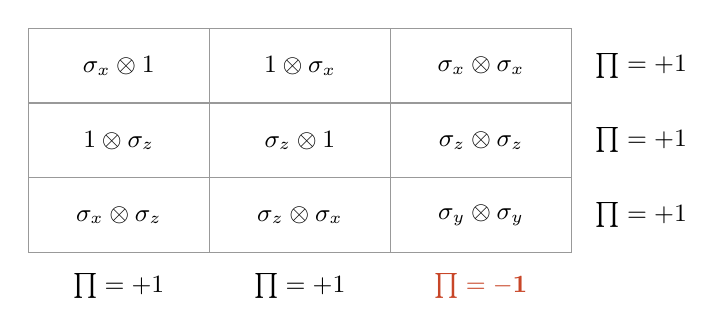
\begin{tikzpicture}[x=2.3cm,y=0.95cm,every node/.style={font=\small}]
\foreach \k in {0,1,2,3} { \draw[black!40] (\k,0) -- (\k,3); \draw[black!40] (0,\k) -- (3,\k); }
\foreach \r/\a/\b/\c in {1/{\sigma_x\otimes 1}/{1\otimes\sigma_x}/{\sigma_x\otimes\sigma_x},
                         2/{1\otimes\sigma_z}/{\sigma_z\otimes 1}/{\sigma_z\otimes\sigma_z},
                         3/{\sigma_x\otimes\sigma_z}/{\sigma_z\otimes\sigma_x}/{\sigma_y\otimes\sigma_y}} {
  \node at (0.5,3.5-\r) {$\a$}; \node at (1.5,3.5-\r) {$\b$}; \node at (2.5,3.5-\r) {$\c$};
  \node[anchor=west] at (3.08,3.5-\r) {$\prod=+1$};
}
\node at (0.5,-0.45) {$\prod=+1$};
\node at (1.5,-0.45) {$\prod=+1$};
\node[text=xcol] at (2.5,-0.45) {$\prod=\mathbf{-1}$};
\end{tikzpicture}
\end{center}
\lean{defs_pm}

\begin{proposition}[Quantum facts]\label{prop:pmq}
Each of the nine observables $A_{ij}$ squares to the identity, so its outcomes are $\pm1$. The three observables in any row, or in any column, commute with each other, so they can be measured together. Their products are
\[
 A_{i1}A_{i2}A_{i3}=+1\ (i=1,2,3),\qquad A_{11}A_{21}A_{31}=A_{12}A_{22}A_{32}=+1,\qquad A_{13}A_{23}A_{33}=-1 .
\]
\end{proposition}
\noindent Lean: \lname{PM_square}, \lname{PM_commute_in_row}, \lname{PM_commute_in_col}, \lname{PM_rows}, \lname{PM_col0}, \lname{PM_col1}, \lname{PM_col2}. Lean checks these by multiplying the $4\times4$ matrices. The sign in the last column comes from $\sigma_x\sigma_z\sigma_y=-i$, which gives $(-i)^2=-1$.
\lean{PM_col2}

\begin{theorem}[Classical impossibility]\label{thm:pmc}
No $3\times3$ array of integers has all row products $+1$ and column products $+1,+1,-1$.
\end{theorem}
\begin{proof}
Multiply all nine entries. Row by row, the product is $(+1)^3=+1$; column by column, it is $(+1)(+1)(-1)=-1$.
\end{proof}
\noindent Lean gives two proofs: the argument above (\lname{classical_square_impossible}), and a check of all $2^9=512$ sign patterns (\lname{classical_square_by_enumeration}), with \texttt{true} standing for $-1$ and exclusive-or for multiplication.
\lean{classical_square_by_enumeration}

\begin{theorem}[Kochen--Specker for two spins]\label{thm:ks}
There is no assignment $\mathrm{val}$ of numbers to observables such that $\mathrm{val}(1)=1$, $\mathrm{val}(-1)=-1$ and, for every row and every column $\{A,B,C\}$ of the square, $\mathrm{val}(ABC)=\mathrm{val}(A)\,\mathrm{val}(B)\,\mathrm{val}(C)$.
\end{theorem}
\begin{proof}
By Proposition~\ref{prop:pmq}, the products are $\pm1$, so the values of the nine entries would form an array forbidden by Theorem~\ref{thm:pmc}.
\end{proof}
\noindent Lean: \lname{kochen_specker_two_spins}.
\lean{kochen_specker_two_spins}

Compared with Section~2, every constraint here involves only commuting observables, i.e.\ quantities that can be measured together, so Bell's defence is no longer available. Quantum mechanics remains consistent (Proposition~\ref{prop:pmq}) because it never assigns the nine values in advance. The outcome for $\sigma_x\otimes\sigma_x$ is not fixed independently of whether it is measured together with row~1 or with column~3. This is \emph{contextuality}.

\section{Summary}
\begin{center}
\renewcommand{\arraystretch}{1.25}
\begin{tabularx}{\textwidth}{>{\raggedright\arraybackslash}p{4.2cm}>{\raggedright\arraybackslash}X>{\raggedright\arraybackslash}X}\toprule
 & \textbf{classical} (sets of states) & \textbf{quantum} (subspaces of a Hilbert space)\\\midrule
``or'' & union & span (Thm.~\ref{thm:unionspan}) \\
``not'' fixed by ``and''/``or'' & yes & no; orthogonality chosen (Prop.~\ref{prop:compl}) \\
$p\vee\neg p$ always true & yes & yes (Thm.~\ref{thm:biv}) \\
a true ``or'' has a true part (bivalence) & yes & no (Thm.~\ref{thm:biv}) \\
distributive law & yes (Thm.~\ref{thm:classical}) & no (Thm.~\ref{thm:fail}); orthomodular law instead (Thm.~\ref{thm:oml}) \\
proof by cases on $q$ & always & only if $p$ is compatible with $q$ (Prop.~\ref{prop:compat}) \\
total probability & yes & no (Prop.~\ref{prop:born}) \\
true/false for all propositions & yes & no (Cor.~\ref{cor:nohv}) \\
pre-assigned values for compatible observables & yes & no for two spins (Thm.~\ref{thm:ks}) \\\bottomrule
\end{tabularx}
\end{center}

\section{Philosophical note: quantum mechanics and Aristotle}
The logic taught for two thousand years under Aristotle's name rests on three principles, usually stated as follows.
\begin{description}
\item[Identity] $p$ is $p$.
\item[Non-contradiction] Nothing can both have and lack the same property at the same time, in the same respect (\emph{Metaphysics}~$\Gamma$.3, 1005b19--20).
\item[Excluded middle] There is nothing between a pair of contradictories. Of any subject, any predicate must either be affirmed or denied (\emph{Metaphysics}~$\Gamma$.7, 1011b23--24).
\end{description}
Aristotle's own wording of the third law is about \emph{things and their properties}, not about formulas. Read this way, it is the left identity of Theorem~\ref{thm:unionspan}: every state either has the property $P$ or has the property $\neg P$. This is the principle quantum mechanics violates. An electron in $\ket{x{+}}$ neither has nor lacks the property $S_z=+\tfrac12$. Of this subject, the predicate can be neither affirmed nor denied.

Measured against the three principles, the balance is:
\begin{itemize}
\item \emph{Identity} is untouched.
\item \emph{Non-contradiction} survives: $P\wedge\neg P=0$ for every $P$ (Theorem~\ref{thm:oml}). No state has and lacks a property at once.
\item \emph{Excluded middle} splits. As a formula with von Neumann's ``or'', $P\vee\neg P$ is always true. As Aristotle states it, about a subject and its predicates, it is false (Theorems~\ref{thm:biv} and~\ref{thm:unionspan}).
\end{itemize}
The two-spin result goes further than the one-spin result. The Peres--Mermin square (Theorem~\ref{thm:ks}) shows that measurement outcomes cannot be properties that a system carries in advance, independent of what else is measured with them. This is a challenge to the ontology behind Aristotle's logic, a world of substances that bear definite attributes. It is not only a challenge to one law of inference. The distributive law that fails in Theorem~\ref{thm:fail} is not Aristotelian at all. It belongs to Boole's algebra of logic (1854), the modern formalisation of the classical tradition.

There is a historical irony. Aristotle himself doubted bivalence in one case, that of future contingents (\emph{De Interpretatione}~9). ``Either there will be a sea battle tomorrow or there will not'' is necessarily true, yet on the usual reading neither part is true today. This is the pattern of Theorem~\ref{thm:biv}: the disjunction is true while neither disjunct is. \L{}ukasiewicz later built a three-valued logic from this passage. Quantum mechanics produces the pattern for present properties, not future events.

Whether quantum mechanics therefore forces a change of \emph{logic} is still debated. Putnam~\cite{Putnam} argued that logic is empirical and that quantum logic is the correct logic of the world. Most physicists and philosophers since then read the Birkhoff--von Neumann lattice as a structure of experimental propositions, with ordinary logic still used to reason \emph{about} it. The Lean file shows the second position in practice: it uses classical reasoning to prove theorems about a non-classical lattice. The topos approach of Section~\ref{sec:ornot} is a third position. It changes the logic, but to the intuitionistic logic, not to the orthomodular one.

\appendix
\section{About the Lean file}
\begin{itemize}
\item \texttt{QuantumLogicSpins.lean} has 59 theorems and lemmas in five parts (0, 0b, 1, 1b, 2) that follow these notes. It compiles against Lean~4.35 and Mathlib with \texttt{lake exe cache get} followed by \texttt{lake build} in the repository \url{https://github.com/alasfar-lina/quantum-logic-spins-lean} (about 40\,s for this file on a laptop, mostly the matrix products).
\item No \texttt{sorry} and no \texttt{native\_decide} are used. \texttt{\#print axioms} reports only Lean's three standard axioms (\texttt{propext}, \texttt{Classical.choice}, \texttt{Quot.sound}), or none.
\item \emph{Lean refuses false statements.} The folder \texttt{mutants/} contains three deliberately wrong claims (one per file; \texttt{mutants/check\_mutants.sh} runs them), and Lean rejects each one. (i) ``Subspaces of $\C^2$ satisfy the distributive law'': Lean cannot find a distributive-lattice structure. (ii) ``The square with all column products $+1$ is impossible'': \texttt{decide} finds the all-$(+1)$ array as a counterexample. (iii) ``The third column multiplies to $+1$'': the matrix check fails. These make a good classroom exercise.
\item Formal choices: the spin space is \texttt{EuclideanSpace ℂ (Fin 2)}, propositions are Mathlib \texttt{Submodule}s, and ``not'' is the orthogonal complement \texttt{ᗮ}. Two-spin observables are Kronecker products \texttt{⊗ₖ} of $2\times2$ complex matrices.
\end{itemize}

\begin{thebibliography}{9}\small
\bibitem{BvN} G.~Birkhoff and J.~von Neumann, \emph{The logic of quantum mechanics}, Ann.\ Math.\ \textbf{37} (1936) 823.
\bibitem{Gleason} A.~M.~Gleason, \emph{Measures on the closed subspaces of a Hilbert space}, J.\ Math.\ Mech.\ \textbf{6} (1957) 885.
\bibitem{Bell} J.~S.~Bell, \emph{On the problem of hidden variables in quantum mechanics}, Rev.\ Mod.\ Phys.\ \textbf{38} (1966) 447.
\bibitem{KS} S.~Kochen and E.~P.~Specker, \emph{The problem of hidden variables in quantum mechanics}, J.\ Math.\ Mech.\ \textbf{17} (1967) 59.
\bibitem{Peres} A.~Peres, \emph{Incompatible results of quantum measurements}, Phys.\ Lett.\ A \textbf{151} (1990) 107.
\bibitem{Mermin} N.~D.~Mermin, \emph{Simple unified form for the major no-hidden-variables theorems}, Phys.\ Rev.\ Lett.\ \textbf{65} (1990) 3373.
\bibitem{Putnam} H.~Putnam, \emph{Is logic empirical?}, in Boston Studies in the Philosophy of Science \textbf{5}, eds.\ R.~S.~Cohen and M.~W.~Wartofsky (Reidel, Dordrecht, 1968) 216.
\bibitem{DI} A.~D\"oring and C.~J.~Isham, \emph{A topos foundation for theories of physics: I.\ Formal languages for physics}, J.\ Math.\ Phys.\ \textbf{49} (2008) 053515.
\bibitem{Landsman} K.~Landsman, \emph{Foundations of Quantum Theory: From Classical Concepts to Operator Algebras} (Springer, Cham, 2017).
\bibitem{EA} M.~Esfahanian and L.~Arntzen, \emph{Exclusion of excluded middle law and quantum mechanics}, arXiv:2303.16076 (2023).
\end{thebibliography}
\end{document}
